\documentclass[twocolumn]{article}

\newcommand{\authorname}{Austin Jetrin Maddison}
\newcommand{\course}{Discrete Simulation}
\newcommand{\courseid}{ICMA393}
\newcommand{\docname}{HW4}
\newcommand{\titletext}{\course: \docname}

%\usepackage{fontspec}	
\usepackage[no-math]{fontspec}	
\setmainfont{HelveticaNowText}
\newfontface\hh{HelveticaNowText-ExtraBold}
\newfontface\lt{HelveticaNowText-Light}      
\newfontface\xx{HelveticaNowText-ExtraLight} 
\newfontface\mm{HelveticaNowText Medium}

\newfontfamily{\displayfont}{HelveticaNowDisplay}
\newfontface\dslt{HelveticaNowDisplay-Light}
\newfontface\dsmm{HelveticaNowDisplay-Medium}
\newfontface\dsbd{HelveticaNowDisplay-Bold}

\newfontfamily{\microfont}{HelveticaNowMicro}
\newfontface\mclt{HelveticaNowMicro-Light}
\newfontface\mcmm{HelveticaNowMicro-Medium}
\newfontface\mcbd{HelveticaNowMicro-Bold}

\setmonofont{SFMono}

\usepackage[lining]{FiraSans}
\usepackage[fakebold]{firamath-otf}
\usepackage{unicode-math}
\setmathfont{FiraMath}
\renewcommand*\oldstylenums[1]{{\firaoldstyle #1}}

\usepackage{microtype}   % Improves text appearance with microtypography
\usepackage{amsmath}     % For better math support
\usepackage{graphicx}    % For including graphics
\usepackage{lipsum}      % For placeholder text
\usepackage{enumitem}
\usepackage{xcolor}
\usepackage{svg}
\usepackage{svg-extract}
\usepackage{caption}
\usepackage{float}
\usepackage{multicol}
\usepackage{booktabs}

\usepackage[a4paper, margin=0.8in, columnsep=20pt]{geometry}

\captionsetup{font=small}
\definecolor{gray}{rgb}{0.55, 0.55, 0.55}
\setlength{\columnsep}{20pt}  % Space between columns

% Headers and Footers
\usepackage{fancyhdr}
\pagestyle{fancy}
\fancyhf{}

% First Page
\fancypagestyle{plain}{
\fancyfoot[R]{\small \thepage} 
\fancyfoot[L]{} 
\fancyhead[L]{}
\fancyhead[R]{}
}

% Custom header
\fancyfoot[L]{\scriptsize \MakeUppercase{ \microfont \courseid~\course}}
\fancyhead[L]{\scriptsize \MakeUppercase{ \microfont \docname}}
\renewcommand{\headrulewidth}{0pt}

% Custom footer
%\fancyfoot[L]{\small Title, Date}
\fancyfoot[R]{\small \thepage}

% Line spacing
\usepackage{setspace}
\setstretch{1.15}  % Slightly more space between lines

%\setlength{\mathindent}{0pt} % This removes the indentation for equations

% Section formatting
\usepackage{titlesec}
\titleformat{\section}[block]{\raggedright \large\dsbd}{\thesection.}{1em}{}
\titleformat{\subsection}[block]{\normalsize \mm}{\thesubsection.}{1em}{}

% Bibliography style
\usepackage[numbers,sort&compress]{natbib} % For numbered citations

% Hyperlinks
\usepackage{hyperref}
\hypersetup{
    colorlinks=false,
    linkcolor=blue,
    citecolor=blue,
    urlcolor=blue,
    pdftitle={Research Paper Title},
    pdfauthor={Author's Name},
}

\usepackage{listings}
\lstset{
  language=Python,                     % Use Python language syntax
  basicstyle=\ttfamily\footnotesize,           % Use modern monospace font for code
  keywordstyle=\bfseries\color{black},   % Bold and blue keywords
  stringstyle=\color{black},              % Strings in red
  commentstyle=\color{gray},            % Comments in gray
  showstringspaces=false,               % Don't show spaces in strings
  breaklines=true,                      % Break long lines
  tabsize=4,                            % Set tab size to 4 spaces
}


\begin{document}
\fontsize{9.5}{11.5}\selectfont % Set font size to 12pt with a baseline of 14pt

% Title 
\title{
  \raggedright
  \Large \displayfont \strong{\courseid~\titletext} \\[5pt]  % Adjust spacing if needed
%  \raggedleft
  \small Mahidol University International College \\
  \small \authorname \\ 
  \small \today
}
\date{} 

%
%\twocolumn[{
%	\vspace*{-1cm}
%	\maketitle
%	\vspace*{-0.5cm}
%}]

\maketitle
%\raggedbottom
\section{Benford’s Law: Chains of Exponential Distributions}

\noindent
I ran the simulation for $N=100000$ iterations, for the $Expo(Expo(Expo(Expo(371))))$.
\vspace{-2pt}
\begin{figure}[H]
	\centering
	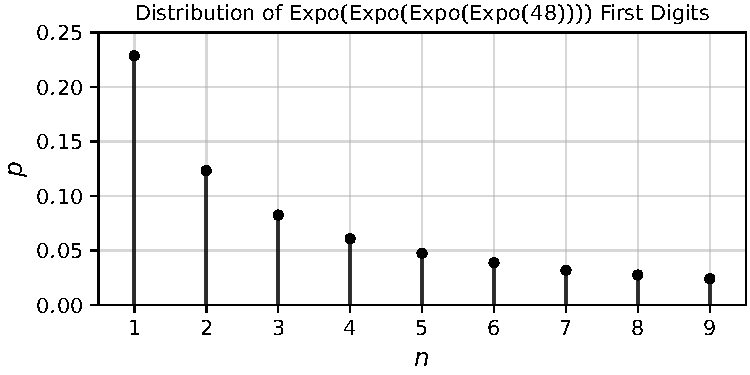
\includegraphics[width=1\linewidth]{../drawings/p1}
	\caption{The chained exponential distributions seems to follow Benford's law.}
	%	\label{fig:path1}
\end{figure}


\section{Inter-Arrival Times Are Independent and Follow the Exponential Distribution}
I ran the simulation for the given intervals for \\$N=100000$ iterations. 
\begin{figure}[H]
	\centering
	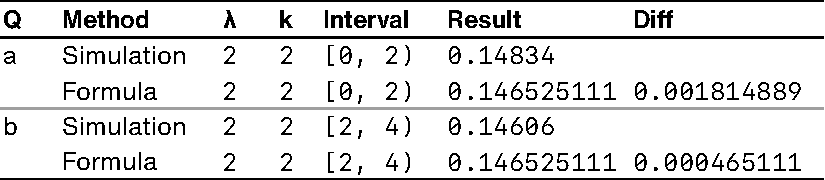
\includegraphics[width=1\linewidth]{../drawings/p2}
	\caption{Comparison of probability results from simulation and theoretical formula for a Poisson process over intervals $[0,2)$ and $[2,4)$}
	%	\label{fig:path1}
\end{figure}

Notice that both simulations a and b have very similar results despite their intervals being different. This is due to the idea that both of their intervals have the same sized "window" that do not change over time (memoryless thing), the length of their intervals are the same. They effectively have the equal chances in this scenario which is quite intuitive, reminds me of roulette wheels.

Now comparing both simulations a and b to the Poisson formula we can see that the formula seems to faithfully model the probability of the scenarios. This is really nice because computing the formula is way faster than iterativley computing the simulation.


\section{Poisson Random Variables}
\section{Exponential Random Variables}

\text{\mm a) Prove that $E[X] = \lambda^{-1}$}
\vspace{-5pt}

\begin{align*}
	= \int_{0}^{\infty} x \cdot \lambda e^{-\lambda x} dx
\end{align*}

Integrate by parts using $\int udv  = uv - \int vdu$, \\let $u = x, dv=\lambda e^{-\lambda x}$.

\begin{align*}
	&= [-xe^{-\lambda x}]_{0}^{\infty} - \int_{0}^{\infty} -e^{-\lambda x} dx\\
	&= [-xe^{-\lambda x}]_{0}^{\infty} - [-\frac{e^{-\lambda x}}{\lambda} ]^{\infty}_{0}\\
	&= [-xe^{-\lambda x}]_{0}^{\infty} - [(-\frac{e^{-\lambda (\infty)}}{\lambda} ) - (-\frac{e^{-\lambda (0)}}{\lambda})] \\
\end{align*}

For the outside term $xe^{-\lambda x} \to 0$, When $x \to \infty$ then $xe^{-\lambda x} \to 0$, and when $x = 0$ then $x e^{-\lambda x} = 0$. Then we evaluate the rest of the equation to get $\lambda^{-1}$

\begin{align*}
	&= 0 -[(0) - (-\frac{1}{\lambda})] \\
	&= \frac{1}{\lambda} = \lambda^{-1}\\
\end{align*}

\noindent
\vspace{-5pt}
\text{\mm b) Prove that $E[E^2] = \lambda^{-2}$}

\vspace{-5pt}
\begin{align*}
	= \int_{0}^{\infty} x^2 \cdot \lambda e^{-\lambda x} dx
\end{align*}

\vspace{-5pt}
Integrate by parts using $\int udv  = uv - \int vdu$, \\let $u = x^2, dv=\lambda e^{-\lambda x}$.

\begin{align*}
    &=[-x^2 e^{-\lambda x}]_{0}^{\infty} + \int_{0}^{\infty} 2x e^{-\lambda x}dx\\
\end{align*}

We learned that the first term $[-x^2 e^{-\lambda x}]_{0}^{\infty}$ evaluates to 0 from computing the last question. 

\begin{align*}
	&=0 +\int_{0}^{\infty}2x e^{-\lambda x}dx\\
\end{align*}

Then I apply integrate by parts again, \\let $u = 2x, dv=e^{-\lambda x} /-\lambda$.
\begin{align*}
	&=[ -\frac{2x}{\lambda} e^{-\lambda x} ]_{0}^{\infty} + \int_{0}^{\infty} \frac{2}{\lambda} e^{-\lambda x}dx\\
	&=0 + \frac{2}{\lambda} \int_{0}^{\infty}  e^{-\lambda x}dx\\
	&= \frac{2}{\lambda} [ -\frac{e^{-\lambda x}}{\lambda} ]_{0}^{\infty} = \frac{1}{\lambda}\\
	&= \frac{2}{\lambda^2} 
\end{align*}


\section{Approximate Exponential Random Value from Tossing a Physical Coin!}
\text{\mm a) Toss your coin 74 times!}

\begin{figure}[H]
	\centering
	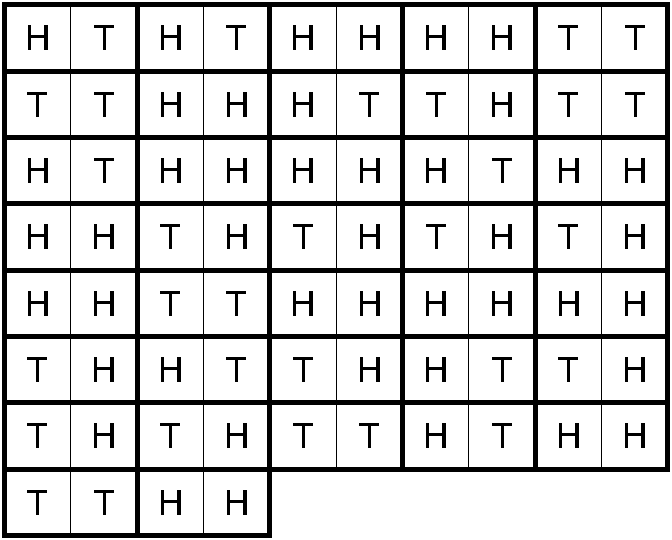
\includegraphics[width=0.65\linewidth]{../drawings/p5}
	\caption{My outcomes recorded of tossing a coin 74 times.}
	%	\label{fig:path1}
\end{figure}
\text{\mm b) Throw away baddies!}
\begin{figure}[H]
	\centering
	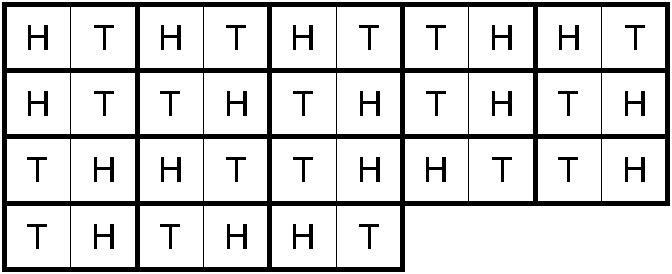
\includegraphics[width=0.65\linewidth]{../drawings/p5.1}
	\caption{18 good pairs.}
	%	\label{fig:path1}
\end{figure}

\text{\mm c) Binary-stringify!}
\begin{align*}
	b_1, b_2, ..., b_{18} = 000100111110101110
\end{align*}

\text{\mm d,e) Compute u and x}

\begin{align*}
	\mathbf{u} = 0.07781410217285156\\
	\mathbf{x} = -log(\mathbf{u}) ≈ 2.553433
\end{align*}



\section{Spooky Buses for Spooktober}

\text{\mm 6.1) Report simulation outputs:} 

\begin{figure}[H]
	\centering
	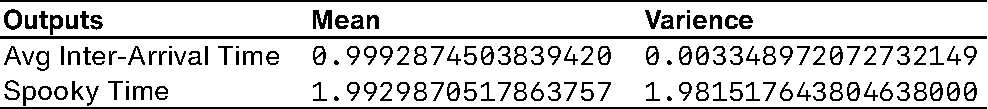
\includegraphics[width=1\linewidth]{../drawings/p6}
	\caption{}
	%	\label{fig:path1}
\end{figure}

\noindent
\text{\mm 6.2) Theoretical Results:} \\\\
Tath really helped me out with this one.\\

\noindent
\mm a) What are the expectation and the variance of the length of the interval that contains t = 163?\\ \normalfont

To frame the simulation by defining $X_1$ and $X_2$ as the pair of buses inter-arrival times that sandwich t=163 st  $X_1$ and $X_2$ are ~Expo(1) and we define T as the total interval length. Then compute E[T]...

\begin{align*}
	E[T] &= E[X_1 + X_2]\\
		 &= E[X_1] + E[X_2]\\
	     &= \frac{1}{\lambda} + \frac{1}{\lambda}\\
	     &= 2
\end{align*}

Then similarly we compute Var[T]...


\begin{align*}
	V[T] &= V[X_1 + X_2]\\
	&= E[X_1] + E[X_2]\\
	&= \frac{1}{\lambda^2} + \frac{1}{\lambda^2}\\
	&= 2
\end{align*}


\noindent
\mm b)  What are the expectation and the variance of the length of the interval between the fifth and the sixth buses? \normalfont\\

Suppose $T_i = X_1 + X_2 ... + X_i$ sum of buses inter arrival times, then we can compute the expected length between buses 5 and 6...
\begin{align*}
	T_6 &= T_5 + X_6\\
	T_6 - T_5 &= X_6\\	
	E[T_6 - T_5] &= E[X_6]\\
	&= \frac{1}{\lambda}\\
	&= 1	
\end{align*}

Again similarly we can compute the variance...
\begin{align*}
	T_6 &= T_5 + X_6\\
	T_6 - T_5 &= X_6\\	
	Var[T_6 - T_5] &= Var[X_6]\\
	&= \frac{1}{\lambda^2}\\
	&= 1	
\end{align*}


\noindent
\mm c) What are the expectation and the variance of the length of the interval between
the last bus before the end (24:00) of October 29 and the first bus after the
beginning (0:00) of October 30? \normalfont\\

I think it would be the same as expectation and variance computed in Q6a. This is because in Q6b we showed that on average the time interval and variance between buses is 1 hour thus and drawing on the memoryless property thing, It said that last bus passed 1 hour ago at most and the bus that is on its way is 1 hour at most. Thus we say that the expected waiting time and variance is 2 hours which lines up with Q6a. 


	


\section*{Source Code}
\href{https://github.com/AustinMaddison/discrete-simulation/tree/main/HW4/source}{https://github.com/AustinMaddison/discrete-simulation/tree/main/hw4/source}

% References
%\bibliographystyle{unsrt}
%\bibliography{references}

\end{document}
